\chapter{Introduction to Cartesian tensor}
\section{Transformation of coordinate frames (Definition of Cartesian tensor)}

Consider two rectangular Cartesian frames 

\begin{align*}
X = \left\{ {0;\tenq{e}_1,\tenq{e}_2,\tenq{e}_3} \right\},
&& 
X' = \left\{ {0;\tenq{e}_1',\tenq{e}_2',\tenq{e}_3'} \right\}
\end{align*} 

\begin{figure}[H]
\centering
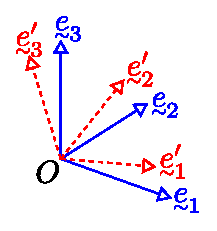
\includegraphics[scale=1.0]{3-1-1.eps}
\caption{Scheme of two rectangular Cartesian frames}
\label{Scheme of two rectangular Cartesian frames-3-1-1}
\end{figure}

Define

\[A_{ij}=\tenq{e}_i'\cdot\tenq{e}_j=\cos(\tenq{e}_i',\tenq{e}_j)=\left(\tenq{e}_i'\right)_j^X=\left(\tenq{e}_j\right)_i^{X'}\]

\[
\tenq{A}=[A_{ij}] = 
\begin{bmatrix}
\tenq{e}_1',\tenq{e}_1 & \tenq{e}_1',\tenq{e}_2 & \tenq{e}_1',\tenq{e}_3 \\ 
\tenq{e}_2',\tenq{e}_1 & \tenq{e}_2',\tenq{e}_2 & \tenq{e}_2',\tenq{e}_3 \\ 
\tenq{e}_3',\tenq{e}_1 & \tenq{e}_3',\tenq{e}_2 & \tenq{e}_3',\tenq{e}_3  
\end{bmatrix}
\]

\[A_{ij}\neq A_{ji}\]

Observed properties 

\[\tenq{e}_p'\cdot\tenq{e}_q'=\delta_{pq}\]

then 

\[A_{pi}A_{qi}=\left(\tenq{e}_p'\right)_i^X\left(\tenq{e}_q'\right)_i^X=\tenq{e}_p'\cdot\tenq{e}_q'\]

\[\Rightarrow \boxed{A_{pi}A_{qi}=\delta_{pq}}\]

Similarly

\[A_{pi}A_{pj}=\left(\tenq{e}_i\right)_p^{X'}\left(\tenq{e}_j\right)_p^{X'}=\tenq{e}_i\cdot\tenq{e}_j\]

\[\Rightarrow \boxed{A_{pi}A_{pj}=\delta_{ij}}\]

in matrix form

\[\tenq{A}\tenq{A}^T=\tenq{A}^T\tenq{A}=\tenq{1}\Rightarrow\tenq{A}=\tenq{A}^{-1}\]

Also

\begin{align*}
\det\tenq{A}
&= \epsilon_{ijk}A_{1i}A_{2j}A_{3k} = \epsilon_{ijk}\left(\tenq{e}_1'\right)_i^X\left(\tenq{e}_2'\right)_j^X\left(\tenq{e}_3'\right)_k^X\\
&= \left(\tenq{e}_1'\wedge\tenq{e}_2'\right)\cdot\tenq{e}_3'
=
\begin{cases}
+1 \text{ right-handed frame}\\
-1 \text{ left-handed frame}
\end{cases}
\end{align*}


\[\therefore\det\tenq{A}=\pm 1\]

$\tenq{A}$ is an \emph{orthogonal} (orthonormal) matrix. \\

If $X\in\mathscr{F}_+$, then $\det\tenq{A}=+1$, $\tenq{A}$ is \emph{proper} matrix.

\begin{notation}\mbox{}\\

The change in coordinate frame $X\to X'$ which is governed by $\tenq{A}$ will be represented as 

\[\tenq{A}\colon X\to X'\]

\end{notation}

Consider a vector $\tenq{v}$

\[\tenq{v}=v_p^X\tenq{e}_p=v_p^{X'}\tenq{e}_p'\]

where 

\begin{align*}
v_p^X &\cdots\text{scalar components of $\tenq{v}$ with respect to frame $X$}\\
v_p^{X'} &\cdots\text{scalar components of $\tenq{v}$ with respect to frame $X'$}
\end{align*}

\[\tenq{v}\cdot\tenq{e}_i'=v_i^{X'}=\left(v_p^X\tenq{e}_p\right)\cdot\tenq{e}_i'=v_p^XA_{ip}\]

\[\Rightarrow\boxed{v_i^{X'}=A_{ip}v_p^X}\]

Similarly

\[\boxed{v_i^X=A_{pi}v_p^{X'}}\]

which are \emph{transformation laws}.

or in matrix form $\tenq{v}=\begin{bmatrix}
v_1^X \\ 
v_2^X\\ 
v_3^X
\end{bmatrix}$\\

$
\left.\begin{aligned}
& \tenq{v}'=\tenq{A}\tenq{v}\\
& \tenq{v}=\tenq{A}^T\tenq{v}'
\end{aligned}\right\}
$ gives confusion, the transformation law only change the \emph{components} of a vector not the vector itself.

\begin{definition}{Definition of vector}\mbox{}\\
A vector is a function defined on all $X$ such that it satisfies the above transformation laws.
\end{definition}

\begin{definition}{Definition of a Cartesian tensor}

Let $N\geq 0$ be an integer. A Cartesian tensor of order $N$ is a function on $\mathscr{F}$ (all $X$) that assigns to each $X\in\mathscr{F}$, an ordered set of $3^N$ real numbers. We will denote

\[V_{\underbrace{ij\cdots k}_{N}}^X\cdots\text{components of $\tenq{V}$ in $X$}\]

such that for every $\tenq{A}\colon X\to X'$ (for every orthogonal transformation which transforms $X$ to $X'$)

\begin{equation}
V_{\underbrace{ij\cdots k}_{N}}^X = A_{ip}A_{jq}\cdots A_{kr}V_{\underbrace{pq\cdots r}_{N}}^X \tag{$\ast$}\label{eq: 3-1-(*)}
\end{equation}

Further, if $\tenq{U}$ and $\tenq{V}$ are both tensors of order $N$ and $c$ is a real number then define

\begin{enumerate}[label=(\roman*)]

\item
$\tenq{U}=\tenq{V}$ if $U_{ij\cdots k}^X=V_{ij\cdots k}^X\phantom{-}\forall X\in\mathscr{F}$

\item \label{ch3-1-def of cart. tensor-(ii)}
$\tenq{W}=\tenq{U}+\tenq{V}$ if $W_{ij\cdots k}^X=U_{ij\cdots k}^X+V_{ij\cdots k}^X\phantom{-}\forall X\in\mathscr{F}$

\item \label{ch3-1-def of cart. tensor-(iii)}
$\tenq{W}=c\tenq{U}$ if $W_{ij\cdots k}^X=cU_{ij\cdots k}^X\phantom{-}\forall X\in\mathscr{F}$

\end{enumerate}

\end{definition}

\begin{note}\mbox{}\\

\begin{enumerate}[label=(\arabic*)]
\item
$V_{ij\cdots k}$ is not a tensor. They are the components of a tensor in a given frame $X$. 

\item
$\tenq{W}$ defined in \ref{ch3-1-def of cart. tensor-(ii)} and \ref{ch3-1-def of cart. tensor-(iii)} is itself a tensor of order $N$.

\item
If $N=0$, $\tenq{V}$ is called a scalar and you write $V$ in place of $\tenq{V}$. 

\item
If $N=1$, $\tenq{V}$ is a vector. 

\item
Equalities needs to be tested for a single frame only.
\end{enumerate}



\end{note}

\begin{definition}\mbox{}\\
A tensor $\tenq{V}$ of order $N\geq 2$ is symmetric/skew symmetric with respect to a pairs of indices of its components if the components of $\tenq{V}$ remain unchanged/change sign under the interchange of these two indices.
\end{definition}


\begin{definition}\mbox{}\\
A tensor is fully symmetric if its is symmetric with respect to any pairs of indices (so as skew symmetric).
\end{definition}


\paragraph{Property}\mbox{}\\

If the component of a tensor are symmetric in one frame then they are symmetric in any other frame

\begin{proof}\mbox{}\\

Let 

\begin{equation}
V_{\cdots i\cdots j\cdots}^X=V_{\cdots j\cdots i\cdots}^X \tag{$\star$}\label{eq: 3-1-star}
\end{equation}

\begin{align*}
V_{\cdots p\cdots q\cdots}^{X'}
&=\cdots A_{pi}\cdots A_{qj}\cdots V_{\cdots i\cdots j\cdots}^X\\
&\vc{=}{\eqref{eq: 3-1-star}}{}{}\cdots A_{qj}\cdots A_{pi}\cdots V_{\cdots j\cdots i\cdots}^X\\
&\vc{=}{\eqref{eq: 3-1-(*)}}{}V_{\cdots q\cdots p\cdots}^{X'}
\end{align*}
\end{proof}

\begin{definition}\mbox{}\\
A tensor $\tenq{V}$ of order $N$ is \emph{isotropic} if its components $V_{ij\cdots k}$ are independents of choice of frame.
\end{definition}

\begin{note}\mbox{}\\

\begin{enumerate}[label=(\arabic*)]

\item
A scalar is an isotropic tensor of order $N=0$. 

\item
The only isotropic vector is the null vector $\tenq{v}=\tenq{0}$.

\end{enumerate}

\end{note}

\begin{claim}\mbox{}\\

\begin{enumerate}[label=(\alph*)]

\item \label{ch3-1-isotropic-claim-(a)}
Let $V_{ij}^X=\delta_{ij}\phantom{-}\footnotemark\forall X\in\mathscr{F}$. $V_{ij}^X$ are the components in frame $X$ of an isotropic second order ($N=2$) tensor. We write $\tenq{V}=\tenq{1}$ (identity tensor).

\item \label{ch3-1-isotropic-claim-(b)}
$V_{ijk}^X=\epsilon_{ijk}\phantom{-}\forall X\in\mathscr{F}_+$. Then $V_{ijk}^X$ are components of an isotropic tensor $\tenq{\epsilon}$ ($N=3$).

\end{enumerate}


\footnotetext{$\forall$, the symbol gives the isotropic property by definition}

\end{claim}

\begin{proof}\mbox{}\\

Sufficient to show that $V_{ij}$ in \ref{ch3-1-isotropic-claim-(a)} and $V_{ij}$ in \ref{ch3-1-isotropic-claim-(b)} are tensor component, i.e. satisfy \eqref{eq: 3-1-(*)}.

\begin{enumerate}[label=(\alph*)]

\item
\[A_{ip}A_{jq}V_{pq}^X=A_{ip}A_{jq}\delta_{ij}=A_{ip}A_{jq}=\delta_{ij}\vc{=}{\text{by}}{\text{def.}}V_{ij}^{X'}\]

\item

\begin{align*}
A_{ip}A_{jq}A_{kr}V_{pqr}^{X}
&=A_{ip}A_{jq}A_{kr}\epsilon_{pqr}=\epsilon_{ijk}\det\tenq{A}\\
&\vc{=}{\footnotemark}{}\epsilon_{ijk} = V_{ijk}^{X'}
\end{align*}



\footnotetext{If $X\in\mathscr{F}_+$, $\det\tenq{A}=+1$}

\end{enumerate}


\end{proof}


From this point on , change notation, denote $\mathscr{F}_+$ by $\mathscr{F}$, i.e. handle only \emph{proper} orthogonal transformation only. 



\begin{claim}\mbox{}\\
\begin{enumerate}[label=(\arabic*)]

\item
Every isotropic tensor of 2\textsuperscript{nd} order is a scalar multiple of $\tenq{1}$. 

\item
Every isotropic tensor of 3\textsuperscript{rd} order is a scalar multiple of $\tenq{\epsilon}$. 

\item
Every isotropic high order tensor can be constructed from $\tenq{1}$ and $\tenq{\epsilon}$. \\
e.g. The most general 4\textsuperscript{th} order isotropic tensor has the form of components

\[C_{ijkl}=\alpha\delta_{ij}\delta_{kl}+\beta\delta_{ik}\delta_{jl}+\gamma\delta_{il}\delta_{jk}\]


where $\alpha$, $\beta$, and $\gamma$ are scalars. 

\end{enumerate}
\end{claim}

\section{Outer multiplication of tensors}

Let $\tenq{U}$ and $\tenq{V}$ be tensor of order $M$ and $N$ respectively. \\

Define 

\[W_{\underbrace{ij\cdots k}_{M}\underbrace{mn\cdots r}_{N}}^X=U_{\underbrace{ij\cdots k}_{M}}^XV_{\underbrace{mn\cdots r}_{N}}^X\phantom{-}\forall X\in\mathscr{F}\]

then $W_{ij\cdots kmn\cdots r}$ are the components of tensor $\tenq{W}$ of order $M+N$ called the outer product of $\tenq{U}$ and $\tenq{V}$ (in that order)

\begin{proof}

\begin{align*}
W_{ij\cdots kmn\cdots r}\vc{=}{\text{by}}{\text{def.}}
&= U_{ij\cdots k}^{X'}V_{mn\cdots r}^{X'} \\
&\vc{=}{\eqref{eq: 3-1-(*)}}{}A_{iI}A_{jJ}\cdots A_{kK}A_{mM}A_{nN}\cdots A_{rR}\underbrace{U_{IJ\cdots K}^XV_{MN\cdots R}^X}_{ 
\vc{=}{\text{by}}{\text{def.}}W_{IJ\cdots KMN\cdots R}^X}
\end{align*}


\end{proof}

\section{Contraction of tensors}

Let $\tenq{U}$ be a tensor of order $N\geq 2$. Let $U_{ij\cdots k}^X$ be its components with $X\in\mathscr{F}$.\\

Define the $3^{N-2}$ real numbers as 

\[V_{\underbrace{ij\cdots k}_{N-2}}^X=U_{\underbrace{ij\cdots r\cdots r\cdots k}_N}^X\phantom{-}X\in\mathscr{F}\]

Then $V_{ij\cdots k}^X$ are components of a new tensor $\tenq{V}$ formed by contraction of $\tenq{U}$.

\begin{proof}\mbox{}\\

Similar to the outer product.

\end{proof}

Let ($N=2$) $U_{ij}^X$ are the components of a 2\textsuperscript{nd} tensor $\tenq{U}$, then 

\[\tenq{V}=U_{rr}^X=U_{11}^X+U_{22}^X+U_{33}^X=\tr \tenq{U}\]

e.g. If $\tenq{U}=\tenq{\sigma}$, the stress tensor, then 

\[\tr \tenq{\sigma}=\sigma_{11}^X+\sigma_{22}^X+\sigma_{33}^X=I_1\]

the 1\textsuperscript{st} invariant of stress tensor.

\section{Operation between tensors}

Let $c$ be a scalar and $\tenq{U}$, $\tenq{V}$ be tensors.\\

Define

\begin{table}[H]
\begin{tabular}{p{4cm}|p{1.2cm}|p{1.2cm}|p{1.2cm}|p{3cm}|p{4cm}}
Definition $\tenq{W}$& order $\tenq{U}$& order $\tenq{V}$& order $\tenq{W}$& Absolute (coordinate-free) notation & Name \\ \hline
$W=U_iV_i$ & 1 & 1 & 0 & $\tenq{W}=\tenq{U}\cdot\tenq{V}$ & dot product betweens two vectors \\ \hline
$W_i=\epsilon_{ijk}U_jV_k$ & 1 & 1 & 1 & $\tenq{W}=\tenq{U}\wedge\tenq{V}$ & cross product \\ \hline
$W_i=U_{ij}V_j$ & 2 & 1 & 1 & $\tenq{W}=\tenq{U}\tenq{V}$ & product \\ \hline
$W_{ijk}=U_{ij}V_k$ & 2 & 1 & 3 & (no notation) & outer product \\ \hline
$W_{ij}=U_{ik}V_{kj}$ & 2 & 2 & 2 & $\tenq{W}=\tenq{U}\tenq{V}$ & 2\textsuperscript{nd} order tensor product \\ \hline
$W_{ij}=U_{i}V_j$ & 1 & 1 & 2 & $\tenq{W}=\tenq{U}\otimes\tenq{V}$ & \emph{Dyadic} or outer product of two vectors \\ \hline
\end{tabular}
\end{table}

\section{Inner product or fully-contracted outer product}


If $\tenq{U}$ and $\tenq{V}$ are both of order $N>0$, define 

\[\tenq{U}\cdot\tenq{V}=U_{ij\cdots k}V_{ij\cdots k}\phantom{-}\]

(no symbol of reference frame needed)\\

Define 

\[\abs{\tenq{U}}=\sqrt{\tenq{U}\cdot\tenq{U}}\]

the \emph{norm} of a tensor $\tenq{U}$.

\begin{claim}{Quotient Rule}

Let 9 real numbers $W_{ij\cdots k}^X$ be defined for all $X\in\mathscr{F}$ (these numbers are not known aprion to be tensor components) and suppose that for any vector $\tenq{u}\neq\tenq{0}$, the 3 real numbers $v_i^X$ defined by 

\begin{align*}
v_i^X=W_{ij}^Xu_j^X
&& 
\forall X\in\mathscr{F}
\end{align*}

are the components in $X$ of a vector $\tenq{v}$. Then $W_{ij}^X$ are components in $X$ of a tensor $\tenq{W}$.

\end{claim}

\begin{proof}\mbox{}\\

By hypothesis, if $\tenq{A}\colon X\to X'$ since both $\tenq{U}$ and $\tenq{V}$ are vectors

\[v_i^X\vc{=}{\eqref{eq: 3-1-(*)}}{}A_{qi}v_q^{X'}\vc{=}{\text{by}}{\text{def.}}W_{ij}^Xu_j^X\vc{=}{\eqref{eq: 3-1-(*)}}{}W_{ij}^X\left(A_{qj}u_q^{X'}\right)\]

multiply by $A_{pi}$

\[
A_{pi}A_{qi}v_q^{X'} = A_{pi}W_{ij}^X A_{qj}u_q^{X'}
\Rightarrow
\delta_{pq}v_q^{X'} = W_{ij}^X A_{pi}A_{qj}u_q^{X'}
\]

\begin{equation}
\Rightarrow
v_p^{X'}=W_{ij}^XA_{pi}A_{qj}u_q^{X'}\tag{1}\label{eq: 3-5-(1)}
\end{equation}

Also by definition


\begin{equation}
v_p^{X'}=W_{pq}^{X'}u_q^{X'}\tag{2}\label{eq: 3-5-(2)}
\end{equation}

\eqref{eq: 3-5-(1)} and \eqref{eq: 3-5-(2)}

\[\left(W_{pq}^{X'}-A_{pi}A_{qj}W_{ij}^X\right)u_q^{X'}=0\]

Choose $\tenq{u}$ such that $u_q^{X'}=\delta_{qs}$ ($s$-fixed)\footnotemark

\footnotetext{choose $\left\{\begin{aligned}
& s=1\to q=1 \\
& s=2\to q=2 \\
& s=3\to q=3 
\end{aligned}\right.$} 

\[\Rightarrow W_{\begin{subarray}{l}
  p1 \\
  \phantom{-}2 \\
  \phantom{-}3
  \end{subarray}}^{X'}-A_{pi}A_{\begin{subarray}{l}
  1j \\
  2\phantom{-} \\
  3\phantom{-}
  \end{subarray}}W_{ij}^X=0\]
  
\[\Rightarrow W_{ps}^{X'}-A_{pi}A_{sj}W_{ij}^X=0\]

i.e. $W_{ij}^X$ obeys transformation law. 



\end{proof}


\section{Product of a second order tensor and a vector}

Let $\tenq{u}$ and $\tenq{v}$ be vectors, $\tenq{W}$ be a 2\textsuperscript{nd} order tensor.\\
Then 

\[\tenq{W}\left(\tenq{u}+\tenq{v}\right)=\tenq{W}\tenq{u}+\tenq{W}\tenq{v}\]

If $X=\left\{0;\tenq{e}_1,\tenq{e}_2,\tenq{e}_3\right\}\in\mathscr{F}$, then 

\[W_{ij}^X=\tenq{e}_i\cdot\left(\tenq{W}\tenq{e}_j\right)\]

the way to find the components of $\tenq{W}$.

\begin{proof}

\begin{align*}
\tenq{e}_i\cdot\left(\tenq{W}\tenq{e}_j\right) 
&= \left(\tenq{e}_i\right)_k\left(\tenq{W}\tenq{e}_j\right)_k = \delta_{ik}\left[W_{kl}\left(\tenq{e}_j\right)_l\right] \\
&= \delta_{ik}W_{kl}\delta_{jl}=W_{ij}
\end{align*}

\end{proof}

\section{Connection between second order tensors and linear vector function (l.v.f.)}

A linear vector function $\tenq{\mathscr{L}}(\bullet)$ is a mapping that assigns to each vector belongs to $E_3$ and other vector $\tenq{v}=\tenq{\mathscr{L}}(\tenq{u})\in E_3$ subjected to the following requirements. 

\begin{enumerate}[label=(\roman*)]

\item
$\tenq{\mathscr{L}}(\tenq{u}^{(1)}+\tenq{u}^{(2)})=\tenq{\mathscr{L}}(\tenq{u}^{(1)})+\tenq{\mathscr{L}}(\tenq{u}^{(2)})$

\item
$\tenq{\mathscr{L}}(c\tenq{u})=c\tenq{\mathscr{L}}(\tenq{u})\phantom{-}\forall c\in\mathbb{R}$

\end{enumerate}

\begin{claim}{Connection of second order tensor to l.v.f.}

\begin{enumerate}[label=(\alph*)]

\item
Let $\tenq{W}$ be a 2\textsuperscript{nd} order tensor and define a function $\tenq{\mathscr{L}}(\bullet)$ as 


\begin{align}
\tenq{v}=\tenq{\mathscr{L}}(\tenq{u}) = \tenq{W}\tenq{u}
&& 
\forall\tenq{u}\in E_3 \tag{$\bigstar$} \label{eq: 3-7-bigstar}
\end{align}

Then $\tenq{\mathscr{L}}$ is a l.v.f.

\item 
Conversely, given a linear vector function $\tenq{\mathscr{L}}(\tenq{u})$, there exists a \emph{unique} 2\textsuperscript{nd} order tensor $\tenq{W}$ such that 

\begin{align*}
\tenq{\mathscr{L}}(\tenq{u}) = \tenq{W}\tenq{u}
&& 
\forall\tenq{u}\in E_3 
\end{align*}

\end{enumerate}

\end{claim}

\begin{proof}\mbox{}\\

\begin{enumerate}[label=(\alph*)]

\item
Recall that $\tenq{W}\left(\tenq{u}+\tenq{v}\right)=\tenq{W}\tenq{u}+\tenq{W}\tenq{v}$

So 

\begin{equation}
\tenq{W}\left(\tenq{u}^{(1)}+\tenq{u}^{(2)}\right)=\tenq{W}\tenq{u}^{(1)} + \tenq{W}\tenq{u}^{(2)} \tag{i} \label{eq: 3-7-i}
\end{equation}

\begin{equation}
\tenq{W}\left(c\tenq{u}\right)=c\tenq{W}\tenq{u} \tag{ii} \label{eq: 3-7-ii}
\end{equation}

\item
Let $\tenq{\mathscr{L}}(\bullet)$ be given. Choose a frame $X=\left\{0;\tenq{e}_1,\tenq{e}_2,\tenq{e}_3\right\}\in\mathscr{F}$. \emph{Let $W_{ji}^X$ be the j\textsuperscript{th} $\tenq{\mathscr{L}}(\tenq{e}_i)$ in frame $X$.}\footnote{Method to find the component of $\tenq{W}$.}

\begin{equation}
\tenq{\mathscr{L}}(\tenq{e}_i)=W_{ji}^X\tenq{e}_j\tag{$\bigstar\bigstar$} \label{eq: 3-7-bigstarbigstar}
\end{equation}

Choose an arbitrary vector $\tenq{u}\in E_3$. Then 

\[\tenq{v}=\tenq{\mathscr{L}}(\tenq{u})=\tenq{\mathscr{L}}(u_i^X\tenq{e}_i)=u_i^X\tenq{\mathscr{L}}(\tenq{e}_i)\vc{=}{\eqref{eq: 3-7-bigstarbigstar}}{}u_i^XW_{ji}^X\tenq{e}_j\]

But $\tenq{v}=v_j^X\tenq{e}_j$

\[\Rightarrow v_j^X=u_i^XW_{ji}^X=W_{ji}^Xu_i^X\vc{=}{i\leftrightarrow j}{}W_{ij}^Xu_j^X\]

By quotient rule, $W_{ij}^X$ are the components of a 2\textsuperscript{nd} order tensor $\tenq{W}$

\[\tenq{v}=\tenq{W}\tenq{u}=\tenq{\mathscr{L}}(\tenq{u})\]

\end{enumerate}

\end{proof}

\paragraph{Uniqueness}\mbox{}\\

Let's assume that exists $\tenq{W}^{(1)}$ and $\tenq{W}^{(2)}$ such that 




\begin{align*}
\left.\begin{aligned}
& \tenq{v}=\tenq{\mathscr{L}}(\tenq{u})= \tenq{W}^{(1)}\tenq{u} \\
& \tenq{v}=\tenq{\mathscr{L}}(\tenq{u})= \tenq{W}^{(2)}\tenq{u} 
\end{aligned}\right\}\Rightarrow\left(\tenq{W}^{(1)}-\tenq{W}^{(2)}\right)\tenq{u}=\tenq{0}
&& 
\forall\tenq{u}\in E_3
\end{align*} 

or 

\[\left(W_{ij}^{(1)}-W_{ij}^{(2)}\right)u_j=0\Rightarrow \tenq{W}^{(1)}=\tenq{W}^{(2)}\]

\begin{note}
Sometimes people define second order tensor by l.v.f.
\end{note}

\section{Transpose of a second order tensor}

Define

\begin{align*}
\tenq{V}=\tenq{U}^T
&& 
\text{if}
&&
V_{ij}=U_{ji}
\end{align*} 

Symmetric 2\textsuperscript{nd} order tensor as one 

\begin{align*}
\tenq{U}=\tenq{U}^T
&& 
\text{or}
&&
U_{ij}=U_{ji}
\end{align*} 

Skew-symmetric 2\textsuperscript{nd} order tensor as one 

\begin{align*}
\tenq{U}=-\tenq{U}^T
&& 
\text{or}
&&
U_{ij}=-U_{ji}
\end{align*} 


If $\tenq{W}$ is a 2\textsuperscript{nd} order tensor and $\tenq{u}$, $\tenq{v}$ are vectors, then 

\[\boxed{\tenq{u}\cdot\left(\tenq{W}\tenq{v}\right)=\left(\tenq{W}^T\tenq{u}\right)\cdot\tenq{v}}\]

\begin{proof}

\begin{align*}
\tenq{u}\cdot\left(\tenq{W}\tenq{v}\right) 
&= u_i\left(\tenq{W}\tenq{v}\right)_i = u_i\left(W_{ij}v_j\right) \vc{=}{i\leftrightarrow j}{}\left(W_{ji}u_j\right)v_i \\
&= \left(\tenq{W}^T\tenq{u}\right)_iv_i = \left(\tenq{W}^T\tenq{u}\right)\cdot\tenq{v}
\end{align*}

\end{proof}

If $\tenq{y}=\tenq{V}\tenq{x}$, $\tenq{z}=\tenq{U}\tenq{y}$ ($\tenq{x},\tenq{y},\tenq{z}\in E_3$, $\tenq{U},\tenq{V}$ are 2\textsuperscript{nd} order tensors)

\begin{align*}
\tenq{z}=\tenq{U}\tenq{V}\tenq{x}
&& 
\text{or}
&&
z_i=U_{ij}V_{jk}x_k
\end{align*} 

\section{Product between two second order tensors}

If $\tenq{U}$ and $\tenq{V}$ are 2\textsuperscript{nd} order tensors, then define 

\begin{align*}
\tenq{W}=\tenq{U}\tenq{V}
&& 
\text{if}
&&
W_{ij}=U_{ik}V_{kj}
\end{align*}

as tensorial product of $\tenq{U}$ and $\tenq{V}$.

\begin{enumerate}[label=(\roman*)]

\item
distribute

\[\tenq{U}\left(\tenq{V}^{(1)}+\tenq{V}^{(2)}\right)=\tenq{U}\tenq{V}^{(1)}+\tenq{U}\tenq{V}^{(2)}\]

\item
associate

\[\left(\tenq{U}\tenq{V}\right)\tenq{W}=\tenq{U}\left(\tenq{V}\tenq{W}\right)\]

\item
non-commutative

\[\tenq{U}\tenq{V}\neq\tenq{V}\tenq{U}\]

\end{enumerate}

If $\tenq{W}=\tenq{U}\tenq{V}$, then 

\[\tenq{W}^T=\tenq{V}^T\tenq{U}^T\]

\begin{proof}

\begin{align*}
W_{ij}=U_{ik}V_{kj} \vc{\Rightarrow}{i\leftrightarrow j}{}W_{ji}
&= U_{jk}V_{ki} \\
&= V_{ki}U_{jk} \\
&= V_{ik}^TU_{kj}^T \\
&= \left(\tenq{V}^T\tenq{U}^T\right)_{ij}
\end{align*}

but $W_{ji}=W_{ij}^T$

\[\therefore\tenq{W}^T=\tenq{V}^T\tenq{U}^T\]

\end{proof}

\section{Tensor (or dyadic) product between two vectors}

If $\tenq{u}$ and $\tenq{v}$ belong to $E_3$, define

\begin{align*}
\tenq{W}=\tenq{u}\otimes \tenq{v}
&& 
\text{if}
&&
W_{ij}=u_{i}v_{j}
\end{align*}

where $\tenq{W}$ is a 2\textsuperscript{nd} order tensor.

\begin{note}\mbox{}\\

\begin{enumerate}[label=(\arabic*)]

\item
\[\tenq{u}\otimes\tenq{v}\neq\tenq{v}\otimes\tenq{u}\]

\item
\[\tenq{u}\otimes\left(\tenq{v}^{(1)}+\tenq{v}^{(2)}\right)=\tenq{u}\otimes\tenq{v}^{(1)} + \tenq{u}\otimes\tenq{v}^{(2)}\]

\item
\[\tenq{W}=\tenq{u}\otimes\tenq{v}\Leftrightarrow\tenq{W}\tenq{a}=\left(\tenq{v}\cdot\tenq{a}\right)\tenq{u}\phantom{-}\forall \tenq{a}\in E_3\]

\end{enumerate}

\begin{proof}\mbox{}\\

\paragraph{$\boxed{\Rightarrow}$}

\[
\tenq{W}\tenq{a}
= \left(W_{ik}a_k\right)\tenq{e}_i = \left(u_iv_ka_k\right)\tenq{e}_i = \left(v_ka_k\right)u_i\tenq{e}_i=\left(\tenq{v}\cdot\tenq{a}\right)\tenq{u}
\]

\paragraph{$\boxed{\Leftarrow}$}

\begin{align*}
\tenq{W}\tenq{a}=\left(\tenq{v}\cdot\tenq{a}\right)\tenq{u}
&& 
\forall\tenq{a}\in E_3
\end{align*}

or 

\[W_{ij}a_j=v_ja_ju_i\]

\[\therefore\left(W_{ij}-u_iv_j\right)a_j=0\]

Since $\tenq{a}$ is arbitrary 

\begin{align*}
W_{ij}=u_iv_j
&& 
\text{or}
&&
\tenq{W}=\tenq{u}\otimes\tenq{v}
\end{align*}


\end{proof}

\end{note}

If $X=\left\{0;\tenq{e}_1,\tenq{e}_2,\tenq{e}_3\right\}\in\mathscr{F}$, then 

\[\boxed{\tenq{W}=W_{ij}^X\tenq{e}_i\otimes\tenq{e}_j}\]

\begin{proof}

\[\tenq{V}=W_{ij}^X\tenq{e}_i\otimes\tenq{e}_j=W_{11}\tenq{e}_1\otimes\tenq{e}_1+W_{12}\tenq{e}_1\otimes\tenq{e}_2+\cdots\]

\begin{align*}
V_{pq}=\left(W_{ij}^X\tenq{e}_i\otimes\tenq{e}_j\right)_{pq}
&= W_{ij}^X\left(\tenq{e}_i\otimes\tenq{e}_j\right)_{pq} \\
&= W_{ij}^X\left(\tenq{e}_i\right)_p\left(\tenq{e}_j\right)_q\\
&= W_{ij}^X\delta_{ip}\delta_{jq} \\
&= W_{pq}^X
\end{align*}

\[\therefore \left(W_{ij}^X\tenq{e}_i\otimes\tenq{e}_j\right)_{pq}=W_{pq}^X\]

or 

\[W_{ij}^X\tenq{e}_i\otimes\tenq{e}_j=\tenq{W}\]

representation theorem of $\tenq{W}$ in terms of a sum of unit vectors of a frame admits components in the same frame.\\

Trace of a 2\textsuperscript{nd} order tensor $\tenq{U}$ as 

\[\tr \tenq{U}=U_{ii}=U_{11}+U_{22}+U_{33}\]

Let $\tenq{U}$ and $\tenq{V}$ be 2\textsuperscript{nd} order tensors, then 

\begin{enumerate}[label=(\arabic*)]

\item
\[\tenq{U}\cdot\tenq{V}=U_{ij}V_{ij}=\tr (\tenq{U}\tenq{V}^T)\]

\item
\[\abs{\tenq{U}}=\sqrt{\tenq{U}\cdot\tenq{U}}=\sqrt{\tr (\tenq{U}\tenq{U}^T)}\]

\item \label{ch3-10-(3)}
\[\det(\tenq{U}\tenq{V})=\det\tenq{U}\det\tenq{V}\]

\begin{proof}
exercise
\end{proof}

\end{enumerate}


\end{proof}

\section{Orthogonal tensors}

A 2\textsuperscript{nd} order tensor $\tenq{Q}$ is orthogonal if $\tenq{Q}\tenq{Q}^T=\tenq{1}$, the identity tensor.

\[\underbrace{\tenq{Q}^{-1}\tenq{Q}}_{\tenq{1}}\tenq{Q}^T=\tenq{Q}^{-1}\Rightarrow\tenq{Q}^T=\tenq{Q}^{-1}\]

or 

\[\det(\tenq{Q}\tenq{Q}^{T})=\det\tenq{1}=1\vc{=}{\ref{ch3-10-(3)}}{}\det\tenq{Q}\det\tenq{Q}^T=\left(\det\tenq{Q}\right)^2\]

\[\Rightarrow\det\tenq{Q}=\pm 1\]

If $\tenq{Q}\tenq{Q}^{T}=\tenq{1}$ and $\det\tenq{Q}=+1$, then $\tenq{Q}$ is called \emph{proper orthogonal}.

\section{Fundamental scalar invariant of a second order tensor}

Let $\tenq{V}$ be a 2\textsuperscript{nd} order tensor. Then define $I_i(\tenq{V})$ as 

\begin{align*}
& I_1(\tenq{V}) = \tr \tenq{V}=V_{ii}=V_{11}+V_{22}+V_{33} \\
& I_2(\tenq{V}) = \frac{1}{2}\left(V_{ii}V_{jj}-V_{ij}V_{ij}\right)=\frac{1}{2}\left[\left(\tr \tenq{V}\right)^2-\tr \tenq{V}^2\right]\\
& I_3(\tenq{V}) = \frac{1}{6}\epsilon_{ijk}\epsilon_{pqr}V_{ip}V_{jq}V_{kr}=\det\tenq{V}
\end{align*}

$I_i(\tenq{V})$ are scalars produced by outer multiplication and contraction and as such as scalars independent of frame.

\begin{definition}\mbox{}\\
A 2\textsuperscript{nd} order tensor $\tenq{V}$ is non-singular if $\det\tenq{V}\neq 0$; otherwise, a 2\textsuperscript{nd} order tensor $\tenq{V}$ is singular if there exists a vector $\tenq{u}\neq \tenq{0}$ such that $\tenq{V}\tenq{u}=\tenq{0}$ or $V_{ij}u_j=0$, then by Cramer's rule $\det[V_{ij}]=0$.
\end{definition}

\begin{claim}\mbox{}\\

\begin{enumerate}[label=(\alph*)]

\item
Let $X=\left\{0;\tenq{e}_1,\tenq{e}_2,\tenq{e}_3\right\}\in\mathscr{F}$. Also let $\tenq{Q}$ be a proper orthogonal tensor and define vectors $\tenq{e}_i'=\tenq{Q}\tenq{e}_i$. Then vector trait $\tenq{e}_i'$ are base vectors for an other proper orthogonal frame $X'=\left\{0;\tenq{e}_1',\tenq{e}_2',\tenq{e}_3'\right\}\in\mathscr{F}$ and the matrix $\tenq{A}$ of direction cosines that transforms $X$ to $X'$ ($\tenq{A}\colon X\to X'$) is given by $A_{ij}=Q_{ji}^X$. 

\item
Let $X=\left\{0;\tenq{e}_1,\tenq{e}_2,\tenq{e}_3\right\}\in\mathscr{F}$ and $X'=\left\{0;\tenq{e}_1',\tenq{e}_2',\tenq{e}_3'\right\}\in\mathscr{F}$ and also let $\tenq{A}\colon X\to X'$ then there exists an \emph{unique} (proper orthogonal) such that $\tenq{e}_i'=\tenq{Q}\tenq{e}_i$ and $\tenq{Q}$ is determined by $Q_{ij}^X=A_{ji}$. 

\end{enumerate}

\end{claim}

\begin{proof}\mbox{}\\

\[\tenq{e}_i'\cdot\tenq{e}_j'=\left(\tenq{Q}\tenq{e}_i\right)\cdot\left(\tenq{Q}\tenq{e}_j\right)\vc{=}{\footnotemark}{}\underbrace{\tenq{Q}^T\tenq{Q}}_{\tenq{1}}\underbrace{\tenq{e}_i\cdot\tenq{e}_j}_{\delta_{ij}}=\delta_{ij}\]

\footnotetext{$\tenq{u}\cdot\left(\tenq{W}\tenq{v}\right)=\left(\tenq{W}^T\tenq{u}\right)\cdot\tenq{v}$}

By definition of $\tenq{A}$

\[\tenq{e}_i'\cdot\tenq{e}_j=A_{ij}\]

\[\therefore A_{ij}=\tenq{e}_i'\cdot\tenq{e}_j=\left(\tenq{Q}\tenq{e}_i\right)\cdot\tenq{e}_j\vc{=}{\footnotemark}{}Q_{ji}^X\]

\footnotetext{$W_{ij}^X=\tenq{e}_i\cdot\left(\tenq{W}\tenq{e}_j\right)$}

\[\det\tenq{A}=\det\tenq{Q}^T=\det\tenq{Q}=+1\]

\end{proof}

\section{Principal value and principal direction of second order tensors definition}

Let $\tenq{V}$ be a second order tensor, a real number $\lambda=\lambda(\tenq{V})$ is a principal value (or an eigenvalue) of $\tenq{V}$ if there exists a vector $\tenq{n}$ such that

\begin{align*}
\tenq{V}\tenq{n}=\lambda\tenq{n}
&& 
\text{and}
&&
\tenq{n}\cdot\tenq{n}=1
\end{align*} 

or 

\begin{align*}
V_{ij}n_j=\lambda n_i
&& 
\text{and}
&&
n_in_i=1
\end{align*} 


If so, $\tenq{n}$ is called a principal direction (or eigenvector) of $\tenq{V}$ corresponding to eigenvalue $\lambda$

\begin{enumerate}

\item

\begin{figure}[H]
\centering
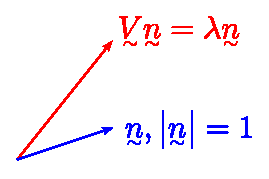
\includegraphics[scale=1.0]{3-13-1-(1).eps}
\caption{Scheme of non-principal direction vector}
\label{Scheme of non-principal direction vector-3-13-1-(1)}
\end{figure}

if $\tenq{n}$ is \emph{not} a principal direction vector.

\item

\begin{figure}[H]
\centering
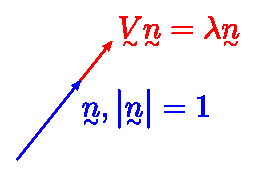
\includegraphics[scale=1.0]{3-13-1-(2).eps}
\caption{Scheme of principal direction vector}
\label{Scheme of principal direction vector-3-13-1-(2)}
\end{figure}

if $\tenq{n}$ is a principal direction vector.


\end{enumerate}

Also $\tenq{n}$ and $-\tenq{n}$ define a principal direction or principal axis belonging to eigenvalue $\lambda$. 


\begin{claim}\mbox{}\\
Let $\tenq{V}$ be a 2\textsuperscript{nd} order tensor. Then $\lambda$ is a principal value of $\tenq{V}$ if and only if it is a real root of the cubic equation

\[F(\lambda)=\det(\tenq{V}-\lambda\tenq{1})=-\lambda^3+I_1(\tenq{V})\lambda^2-I_2(\tenq{V})\lambda+I_3(\tenq{V})=0\]

which is characteristic equation of $\tenq{V}$. \\

If $\lambda$ is a principal value of $\tenq{V}$, then the principal direction vector belonging to $\lambda$ are the solutions for $\tenq{n}$ of the equations

\[
\left\{\begin{aligned}
& \left(V_{ij}-\lambda\delta_{ij}\right)n_j=0 \\
& n_in_i=1
\end{aligned}\right.
\]

\begin{note}
Every 2\textsuperscript{nd} order tensor has at least one real eigenvalue (since a cubic of real coefficient has at least one real root). If the other roots are complex, they are complex conjugate. 
\end{note}


\begin{proof}\mbox{}\\

Let $\lambda$ be eigenvalue, then there exists 3 real numbers $n_i$, not all zeros such that

\[V_{ij}n_j-\lambda n_i=0\]

or 

\[\left(V_{ij}-\lambda\delta_{ij}\right)n_j=0\]

From Cramer's Rule

\[\det(V_{ij}-\lambda\delta_{ij})=0\]

(for non-trivial solution)

\[\det(V_{ij}-\lambda\delta_{ij})=\frac{1}{6}\epsilon_{ijk}\epsilon_{pqr}\left(V_{ip}-\lambda\delta_{ip}\right)\left(V_{jq}-\lambda\delta_{jq}\right)\left(V_{kr}-\lambda\delta_{kr}\right)=0\]

(by definition of invariants)

\[\Rightarrow -\lambda^3+I_1(\tenq{V})\lambda^2-I_2(\tenq{V})\lambda+I_3(\tenq{V})=0\]

\end{proof}

\end{claim}

\section{Symmetric tensors for second order tensors}

\begin{theorem}\label{ch3-14-thm.}\mbox{}\\

Let $\tenq{V}=\tenq{V}^T$, then all three roots ($\lambda_1,\lambda_2,\lambda_2$) of the characteristic equation are real. 

\begin{equation}
F(\lambda)=\det(\tenq{V}-\lambda\tenq{1})=-\lambda^3+I_1\lambda^2-I_2\lambda+I_3=0 \tag{i}\label{eq: 3-14-(i)}
\end{equation}

Further, there exists \emph{at least} one set of three mutually perpendicular principal axes of $\tenq{V}$ and if $X'=\left\{0;\tenq{e}_1',\tenq{e}_2',\tenq{e}_3'\right\}\in\mathscr{F}$ is a principal frame for $\tenq{V}$ then one has

\begin{align*}
[V_{ij}^{X'}]
=
\begin{bmatrix}
\lambda_1 & 0 & 0 \\ 
0 & \lambda_2 & 0 \\ 
0 & 0 & \lambda_3  
\end{bmatrix}
&& 
\text{or}
&&
V_{ij}^{X'}=\lambda_i\delta_{ij}\phantom{-}\text{(no sum)}
\end{align*} 

provided that

\begin{align*}
\tenq{V}\tenq{e}_i'=\lambda_i\tenq{e}_i'
&& 
\text{(no sum)}
\end{align*} 

i.e. $\tenq{e}_i'$ are principal direction vectors.


\begin{enumerate}[label= \fbox{Case \Roman*}]

\item
($\lambda_1,\lambda_2,\lambda_3$) are distinct roots of \eqref{eq: 3-14-(i)} (simple roots) then there exists a unique principal axis belonging to each principal value $\lambda_i$ and the three principal axes are mutually perpendicular. 

\item
Say $\lambda_1\neq\lambda_2=\lambda_3=\lambda_\ast$, i.e. \eqref{eq: 3-14-(i)} has one simple root and a double root. Then there exists a unique principal axis belonging to $\lambda_1$ and every axis which is perpendicular to the former is a principal axis belonging to $\lambda_\ast$. 

\item
$\lambda_1=\lambda_2=\lambda_3=\lambda_\ast$, i.e. \eqref{eq: 3-14-(i)} has a triple root. Then every axis is a principal axis belonging to $\lambda_\ast$ and 

\begin{align*}
\tenq{V}=\lambda_\ast\tenq{1}
&& 
\text{or}
&&
V_{ij}=\lambda_\ast\delta_{ij}
&&
\forall X\in\mathscr{F}
\end{align*} 

so $\tenq{V}$ is an isotropic tensor. 


\end{enumerate}


\end{theorem}

\begin{lemma}\label{ch3-14-lemma 1}\mbox{}\\

If $\tenq{n}^{(1)}$ and $\tenq{n}^{(2)}$ are principal direction vectors belonging to two \emph{distinct} principal values $\lambda_1$ and $\lambda_2$, then $\tenq{n}^{(1)}\perp\tenq{n}^{(2)}$. 

\end{lemma}

\begin{proof}\mbox{}\\

\begin{equation}
\left\{\begin{aligned}
& \tenq{V}\tenq{n}^{(1)}=\lambda_1\tenq{n}^{(1)} \\
& \tenq{V}\tenq{n}^{(2)}=\lambda_2\tenq{n}^{(2)}
\end{aligned}\right.\text{ where }\tenq{V}=\tenq{V}^T\tag{$\circledS$}\label{eq: 3-14-circledS}
\end{equation}

\begin{align*}
\tenq{n}^{(2)}\cdot\lambda_1\tenq{n}^{(1)}
&\vc{=}{\eqref{eq: 3-14-circledS}}{}\tenq{n}^{(2)}\cdot\tenq{V}\tenq{n}^{(1)}\vc{=}{\footnotemark}{}\left(\tenq{V}^T\tenq{n}^{(2)}\right)\cdot\tenq{n}^{(1)}\\
&\vc{=}{\tenq{V}^T=\tenq{V}}{}\tenq{V}\tenq{n}^{(2)}\cdot\tenq{n}^{(1)}\vc{=}{\eqref{eq: 3-14-circledS}}{}\lambda_2\tenq{n}^{(2)}\cdot\tenq{n}^{(1)}
\end{align*}


\footnotetext{$\tenq{u}\cdot\left(\tenq{W}\tenq{v}\right)=\left(\tenq{W}^T\tenq{u}\right)\cdot\tenq{v}$}

\[\Rightarrow\left(\lambda_1-\lambda_2\right)\tenq{n}^{(2)}\cdot\tenq{n}^{(1)}=0\]

\[\vc{\Rightarrow}{\lambda_1\neq\lambda_2}{}\tenq{n}^{(2)}\cdot\tenq{n}^{(1)}=0\text{ or }\tenq{n}^{(2)}\perp\tenq{n}^{(1)}\]

\end{proof}

\begin{lemma}\label{ch3-14-lemma 2}\mbox{}\\

Let $\lambda$ be a principal value of a symmetric, 2\textsuperscript{nd} order tensor $\tenq{V}$ and $\tenq{n}$ be a principal vector belonging to $\lambda$. For fixed $k$ ($k=1,2,3$), choose $X=\left\{0;\tenq{e}_1,\tenq{e}_2,\tenq{e}_3\right\}\in\mathscr{F}$ in such a way that $\tenq{e}_k=\tenq{n}$, i.e. $\tenq{V}\tenq{n}=\lambda\tenq{n},\tenq{V}\tenq{e}_k=\lambda\tenq{e}_k$. Then 

\[V_{ki}^X=V_{ik}^X=\lambda\delta_{ik}\]

e.g. $k=1$

\[V_{ki}^X
=
\begin{bmatrix}
\lambda & 0 & 0 \\ 
0 & V_{22}^X & V_{23}^X \\ 
0 & V_{32}^X & V_{33}^X  
\end{bmatrix}
\]

\end{lemma}

\begin{proof}\mbox{}\\

Choose and fix $k$. By hypothesis

\[\tenq{V}\tenq{e}_k=\lambda\tenq{e}_k\Rightarrow V_{ij}^X\left(\tenq{e}_k\right)_j=\lambda\left(\tenq{e}_k\right)_i\Rightarrow V_{ij}^X\delta_{kj}=\lambda\delta_{ki}\]

\[\Rightarrow V_{ki}^X=\lambda\delta_{ki}\]

\end{proof}

\begin{proof}{Proof of theorem \ref{ch3-14-thm.}}

Let $\tenq{n}^{(1)}$ be a principal direction vector belonging to $\lambda_1$. Choose frame $X'=\left\{0;\tenq{e}_1',\tenq{e}_2',\tenq{e}_3'\right\}\in\mathscr{F}$ that $\tenq{e}_1'=\tenq{n}^{(1)}$. Then by lemma \ref{ch3-14-lemma 2} 

\begin{align}
\tenq{V}_{1i}^{X'}=\lambda_1\delta_{i1}
&& 
\text{or}
&&
V_{11}^{X'}=\lambda_1,V_{12}^{X'}=V_{21}^{X'}=V_{13}^{X'}=V_{31}^{X'}=0
\tag{a}\label{eq: 3-14-pf.-a}
\end{align} 

Thus 

\[\det(V_{ij}^{X'}-\lambda\delta_{ij})=\det
\begin{bmatrix}
\lambda_1-\lambda & 0 & 0 \\ 
0 & V_{22}^{X'}-\lambda &  V_{23}^{X'}-\lambda \\ 
0 & V_{32}^{X'}-\lambda &  V_{33}^{X'}-\lambda  
\end{bmatrix}=0
\]

\begin{equation}
\Rightarrow\left(\lambda_1-\lambda\right)\left\{\lambda^2-\left(V_{22}^{X'}+V_{33}^{X'}\right)\lambda+V_{22}^{X'}V_{33}^{X'}-\left(V_{23}^{X'}\right)^2\right\}=0\tag{b}\label{eq: 3-14-pf.-b}
\end{equation}



\begin{equation}
\left.\begin{aligned}
 \therefore \lambda&=\lambda_1 \\
 \lambda&=
\begin{pmatrix}
\lambda_2 \\
\lambda_3 
\end{pmatrix}\\
&=\frac{V_{22}^{X'}+V_{33}^{X'}}{2}\\
&\pm\underbrace{\sqrt{\frac{\left(V_{22}^{X'}+V_{33}^{X'}\right)-4\left[V_{22}^{X'}V_{33}^{X'}-\left(V_{23}^{X'}\right)^2\right]}{4}}}_{\sqrt{\frac{\left(V_{22}^{X'}-V_{33}^{X'}\right)^2}{4}+\left(V_{23}^{X'}\right)^2}}
\end{aligned}\right.\tag{c}\label{eq: 3-14-pf.-c}
\end{equation}

the roots are real roots.

\begin{enumerate}[label= \fbox{Case \Roman*}]

\item $\lambda_1,\lambda_2,\lambda_3$ are distinct\\

Let $\tenq{n}^{(i)}$ be the three principal axes belonging to $\lambda_i$ by lemma \ref{ch3-14-lemma 1}, $\tenq{n}^{(i)}$ are mutually perpendicular. Let $X'=\left\{0;\tenq{e}_1',\tenq{e}_2',\tenq{e}_3'\right\}\in\mathscr{F}$ such that $\tenq{n}^{(1)}=\tenq{e}_1'$, $\tenq{n}^{(2)}=\tenq{e}_2'$, $\tenq{n}^{(3)}=\tenq{e}_3'$. By lemma \ref{ch3-14-lemma 2} for $k=1,2,3$

\begin{align*}
\left.\begin{aligned}
& V_{i1}^{X'}=\lambda_1\delta_{i1}\\
& V_{i2}^{X'}=\lambda_2\delta_{i2}\\
& V_{i3}^{X'}=\lambda_3\delta_{i3}
\end{aligned}\right\}V_{ij}^{X'}=\lambda_j\delta_{ij}
&&
\text{(no sum)}
\end{align*}

i.e.

\[[V_{ij}^{X'}]=
\begin{bmatrix}
\lambda_1 & 0 & 0 \\ 
0 & \lambda_2 & 0 \\ 
0 & 0 & \lambda_3  
\end{bmatrix}
\]

\item $\lambda_1\neq\lambda_2=\lambda_3=\lambda_\ast$\\

Choose $X'=\left\{0;\tenq{e}_1',\tenq{e}_2',\tenq{e}_3'\right\}\in\mathscr{F}$ such that $\tenq{e}_1'=\tenq{n}^{(1)}$ then \eqref{eq: 3-14-pf.-a} holds, i.e. $V_{11}^{X'}=\lambda_1$, $V_{12}^{X'}=V_{21}^{X'}=V_{13}^{X'}=V_{31}^{X'}=0$. In addition, $\lambda_2=\lambda_3=\lambda_\ast$

\begin{equation}
\vc{\Rightarrow}{\eqref{eq: 3-14-pf.-c}}{}V_{22}^{X'}=V_{33}^{X'}=\lambda_\ast,V_{23}^{X'}=V_{32}^{X'}=0 \tag{d}\label{eq: 3-14-pf.-d}
\end{equation}

i.e. 

\[[V_{ij}^{X'}]=
\begin{bmatrix}
\lambda_1 & 0 & 0 \\ 
0 & \lambda_\ast & 0 \\ 
0 & 0 & \lambda_\ast  
\end{bmatrix}
\]

To show that any choice of $\tenq{e}_2'$, $\tenq{e}_3'$ ($\perp\tenq{n}^{(1)}$) is principal axis

\[\left(\tenq{V}\tenq{e}_2'\right)_i=V_{ij}^{X'}\left(\tenq{e}_2'\right)_j=V_{ij}^{X'}\delta_{2j}=V_{i2}^{X'}=\lambda_\ast\delta_{i2}=\lambda_\ast\left(\tenq{e}_2'\right)_i\]

\[\therefore \tenq{V}\tenq{e}_2'=\lambda_\ast\tenq{e}_2'\]

Similarly

\[
\tenq{V}\tenq{e}_3'=\lambda_\ast\tenq{e}_3'
\]

\begin{figure}[H]
\centering
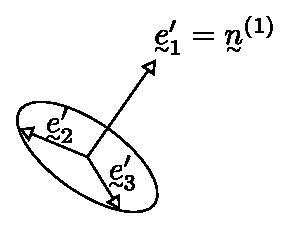
\includegraphics[scale=1.0]{3-14-1.eps}
\caption{Scheme of eigenvectors of $\lambda_1\neq\lambda_2=\lambda_3=\lambda_\ast$}
\label{Scheme of eigenvectors of l1,l2,l3-3-14-1}
\end{figure}

infinite choice of $\tenq{e}_2'$ and $\tenq{e}_3'$. 

\item $\lambda_1=\lambda_2=\lambda_3=\lambda_\ast$\\
Choose $X'=\left\{0;\tenq{e}_1',\tenq{e}_2',\tenq{e}_3'\right\}\in\mathscr{F}$ such that $\tenq{e}_1'=\tenq{n}^{(1)}$ (one eigenvector belonging to $\lambda_1=\lambda_\ast$). Then \eqref{eq: 3-14-pf.-a} holds and \eqref{eq: 3-14-pf.-d} holds, i.e. 

\begin{align*}
[V_{ij}^{X'}]=
\begin{bmatrix}
\lambda_\ast & 0 & 0 \\ 
0 & \lambda_\ast & 0 \\ 
0 & 0 & \lambda_\ast  
\end{bmatrix}
&&
\text{or}
&&
V_{ij}^{X'}=\lambda_\ast\delta_{ij}
&&
\text{or}
&&
\tenq{V}=\lambda_\ast\tenq{1}
\end{align*}

\[\Rightarrow\tenq{V}\tenq{n}=\lambda_\ast\tenq{1}\tenq{n}=\lambda_\ast\tenq{n}\]

where $\tenq{n}$ is any unit vector vector. \\

Every unit vector $\tenq{n}$ is a principal direction vector belonging to $\lambda_\ast$ and every frame $X\in\mathscr{F}$ is a principal frame for $\tenq{V}$. 


\end{enumerate}



\end{proof}

\begin{theorem}{Spectral Representation theorem}

Let $X' = \left\{ {0;\tenq{e}_1',\tenq{e}_2',\tenq{e}_3'} \right\}\in\mathscr{F}$ is a principal frame for a symmetric 2\textsuperscript{nd} tensor $\tenq{V}$ and let $\lambda_i$ be the eigenvectors. Then 

\[\tenq{V}=\sum_{i=1}^3\lambda_i\tenq{e}_i'\otimes\tenq{e}_i'=\lambda_1\tenq{e}_1'\otimes\tenq{e}_1'+\lambda_2\tenq{e}_2'\otimes\tenq{e}_2'+\lambda_3\tenq{e}_3'\otimes\tenq{e}_3'\]

\end{theorem}

\begin{proof}\mbox{}\\

Recall that for all $X\in\mathscr{F}$, not necessary principal

\[\tenq{V}=V_{ij}^X\tenq{e}_i\otimes\tenq{e}_j\]

if we choose a principal frame $X' = \left\{ {0;\tenq{e}_1',\tenq{e}_2',\tenq{e}_3'} \right\}\in\mathscr{F}$, then $V_{ij}^{X'}=\lambda_i\delta_{ij}\phantom{-}\text{(no sum)}$\\

So 

\begin{align*}
\tenq{V}
&= V_{11}^{X'}\tenq{e}_1'\otimes\tenq{e}_1'+V_{12}^{X'}\tenq{e}_1'\otimes\tenq{e}_2'+V_{13}^{X'}\tenq{e}_1'\otimes\tenq{e}_3'+\cdots \\
&= \lambda_1\tenq{e}_1'\otimes\tenq{e}_1'+0+0+\cdots \\
&= \lambda_1\tenq{e}_1'\otimes\tenq{e}_1'+\lambda_2\tenq{e}_2'\otimes\tenq{e}_2'+\lambda_3\tenq{e}_3'\otimes\tenq{e}_3'
\end{align*}

\end{proof}

If $\lambda_1\neq\lambda_2=\lambda_3=\lambda_\ast$, then 

\[\tenq{V}=\left(\lambda_1-\lambda_\ast\right)\tenq{e}_1'\otimes\tenq{e}_1'+\lambda_\ast\tenq{1}\footnotemark\]

\footnotetext{$\displaystyle\because\tenq{1}=\sum_{j=1}^3\tenq{e}_j'\otimes\tenq{e}_j'$ (Homework)}

If $\lambda_1=\lambda_2=\lambda_3=\lambda_\ast$, then 

\[\tenq{V}\lambda_\ast\tenq{1}\]


\section{Skew-symmetric tensors for second order tensors}

\begin{align*}
\tenq{V}=-\tenq{V}^T
&& 
\text{or}
&&
V_{ij}=-V_{ji}
\end{align*} 

\[[V_{ij}]=
\begin{bmatrix}
0 & V_{12} & V_{13} \\ 
-V_{12} & 0 & V_{23} \\ 
-V_{13} & -V_{23} & 0  
\end{bmatrix}\Rightarrow\det\tenq{V}=0
\]

every skew-symmetric tensor is \emph{singular}. \\

Three number $V_{12}$, $V_{13}$, $V_{23}$ are needed to define a skew symmetric tensor. \\

Define a vector $\tenq{w}$ as follows

\begin{align}
\tenq{w}=\textit{dual }\tenq{V}
&& 
\text{if}
&&
w_i=\frac{1}{2}\epsilon_{ijk}V_{kj}\tag{$\star$} \label{eq: 3-15-star}
\end{align} 

The component $V_{ij}$ of $\tenq{V}$ are related to $\tenq{w}$ by 

\begin{align*}
V_{ij}=\epsilon_{ikj}w_k
&& 
\text{or}
&&
[V_{ij}]=
\begin{bmatrix}
0 & -\omega_3 & -\omega_2 \\ 
\omega_3 & 0 & -\omega_1 \\ 
\omega_2 & \omega_1 & 0  
\end{bmatrix}
\end{align*} 

\begin{proof}\mbox{}\\

From \eqref{eq: 3-15-star}

\[w_i=\frac{1}{2}\epsilon_{ijk}V_{kj}\]

multiply both side by $-\epsilon_{ipq}$

\begin{align*}
-\epsilon_{ipq}w_i 
&= -\frac{1}{2}\epsilon_{ipq}\epsilon_{ijk}V_{kj} \\
&= -\frac{1}{2}\left(\delta_{pj}\delta_{qk}-\delta_{pk}\delta_{qj}\right)V_{kj} \\
&= -\frac{1}{2}\left(V_{qp}-V_{pq}\right)=V_{pq}
\end{align*}

\[\therefore V_{pq}=\epsilon_{piq}w_i\vc{\Rightarrow}{i\to k}{\begin{subarray}{l}
  p\to i \\
  q\to j
  \end{subarray}}V_{ij}=\epsilon_{ikj}w_k\]
  
\end{proof}
  
If $\tenq{V}$ is skew-symmetric and $\tenq{w}=\textit{dual }\tenq{V}$, then 

\[\boxed{\tenq{V}\tenq{u}=\tenq{w}\wedge\tenq{u}\phantom{-}\forall\tenq{u}\in E_3}\]

\begin{proof}\mbox{}\\

\[\left(\tenq{w}\wedge\tenq{u}\right)_i=\underbrace{\epsilon_{ikj}w_k}_{V_{ij}}u_j = V_{ij}u_j=\left(\tenq{V}\tenq{u}\right)_i\]



\end{proof}

\section{Decomposition Theorem for second order tensors}

\begin{claim}\mbox{}\\
Every 2\textsuperscript{nd} order tensor $\tenq{W}$ admits a \emph{unique} decomposition such that

\begin{equation}
\tenq{W}=\tenq{U}+\tenq{V}\tag{$\ast$}\label{eq: 3-15-*}
\end{equation}

where 

\begin{alignat*}{3}
& \tenq{U}     \quad && \colon\text{symmetric } \quad && (\tenq{U}=\tenq{U}^T)\\
& \tenq{V}     \quad && \colon\text{skew-symmetric } \quad && (\tenq{V}=-\tenq{V}^T)
\end{alignat*}



Further this resolution is 

\begin{equation}
\left\{\begin{aligned}
& \tenq{U}=\frac{1}{2}\left(\tenq{W}+\tenq{W}^T\right) \\
& \tenq{V}=\frac{1}{2}\left(\tenq{W}-\tenq{W}^T\right) 
\end{aligned}\right.\tag{$\ast\ast$}\label{eq: 3-15-**}
\end{equation}

or 

\[
\left\{\begin{aligned}
& U_{ij}=\frac{1}{2}\left(W_{ij}+W_{ji}\right) \\
& V_{ij}=\frac{1}{2}\left(W_{ij}-W_{ji}\right) 
\end{aligned}\right.
\]

\begin{align*}
\tenq{U}=\textit{sym }\tenq{W}
&& 
\tenq{V}=\textit{skew }\tenq{W}
\end{align*}



\end{claim}

\begin{claim}{Isotropic tensors of 1\textsuperscript{st} and 2\textsuperscript{nd} order tensor}

\begin{enumerate}[label=(\alph*)]

\item\label{ch3-16-claim-(a)}
If $\tenq{v}$ is an isotropic vector, then $\tenq{v}=\tenq{0}$. 
\item\label{ch3-16-claim-(b)}
If $\tenq{V}$ is an isotropic \emph{skew-symmetric} 2\textsuperscript{nd} order tensor, then $\tenq{V}=\tenq{0}$.
\item
If $\tenq{V}$ is an isotropic 2\textsuperscript{nd} order tensor, then $\tenq{V}=\alpha\tenq{1}$, $\alpha\in\mathbb{R}$. 

\end{enumerate}

\end{claim}

\begin{proof}\mbox{}\\

\begin{enumerate}[label=(\alph*)]

\item
$\tenq{v}$ is an isotropic vector, choose $X=\left\{0;\tenq{e}_1,\tenq{e}_2,\tenq{e}_3\right\}\in\mathscr{F}$, $\tenq{v}=v_i^X\tenq{e}_i$. Construct $X'=\left\{0;\tenq{e}_1',\tenq{e}_2',\tenq{e}_3'\right\}=\left\{0;\tenq{e}_1,\tenq{e}_3,-\tenq{e}_2\right\}$.

\begin{figure}[H]
\centering
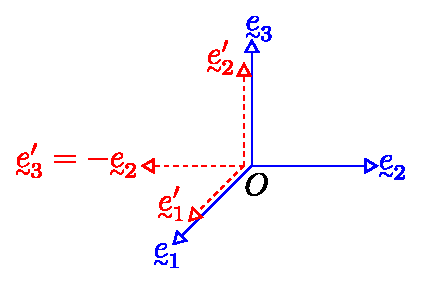
\includegraphics[scale=1.0]{3-16-1.eps}
\caption{Scheme of frame $X'$}
\label{Scheme of frame Xp-3-16-1}
\end{figure}

$X'$ obtained from $X$ by rotation about $\tenq{e}_1$ axis (angle: $\pi/2$)\\

Define $X''=\left\{0;\tenq{e}_1'',\tenq{e}_2'',\tenq{e}_3''\right\}\in\mathscr{F}$ by rotation of $X$ through $\pi/2$ about $\tenq{e}_1$ axis, i.e. $X''=\left\{0;\tenq{e}_1'',\tenq{e}_2'',\tenq{e}_3''\right\}=\left\{0;-\tenq{e}_3,\tenq{e}_2,\tenq{e}_1\right\}$.\\

By the definition of isotropic tensor

\[
\begin{bmatrix}
v_1 \\ 
v_2 \\ 
v_3  
\end{bmatrix}_{X}
=
\begin{bmatrix}
\tenq{v}\cdot\tenq{e}_1'=\tenq{v}\cdot\tenq{e}_1= v_1 \\ 
\tenq{v}\cdot\tenq{e}_2'=\tenq{v}\cdot\tenq{e}_3= v_3 \\ 
\tenq{v}\cdot\tenq{e}_3'=\tenq{v}\cdot\left(-\tenq{e}_2\right)= -v_2  
\end{bmatrix}_{X'}
=
\begin{bmatrix}
-v_3 \\ 
v_2 \\ 
v_1  
\end{bmatrix}_{X''}
\]

\[\Rightarrow
\left\{\begin{aligned}
& v_1=-v_3 \\
& v_3=v_2 \\
& -v_2=v_1 
\end{aligned}\right.\]

\[\Rightarrow v_1=v_2=v_3=0\]

\item
Let $\tenq{V}=-\tenq{V}^T$ and be isotropic

\[\tenq{w}=\textit{dual }\tenq{V}\]

or 

\[w_i=\frac{1}{2}\underbrace{\epsilon_{ijk}}_{\text{isotropic}} \underbrace{V_{kj}}_{\begin{subarray}{l}
  \text{isotropic} \\
  \text{by hypothesis}
  \end{subarray}}\Rightarrow\tenq{w}\text{ is isotropic}\vc{=}{\ref{ch3-16-claim-(a)}}{}\tenq{w}=0 \]
  
\[\Rightarrow\tenq{V}=\tenq{0}\]

\item
Let $\tenq{V}\neq 0$ be an isotropic tensor, then both $\textit{sym }\tenq{V}$ and $\textit{skew }\tenq{V}$ are isotropic. By \ref{ch3-16-claim-(b)} $\textit{skew }\tenq{V}=\tenq{0}$, thus 


\begin{align*}
\tenq{V}=\textit{sym }\tenq{V}
&& 
\text{or}
&&
\tenq{V}=\tenq{V}^T
\end{align*} 

i.e. any non-zero isotropic tensor is symmetric. \\

Thus there exists a frame $X=\left\{0;\tenq{e}_1,\tenq{e}_2,\tenq{e}_3\right\}\in\mathscr{F}$ such that

\begin{align*}
[V_{ij}^X]
=
\begin{bmatrix}
\lambda_1 & 0 & 0 \\ 
0 & \lambda_2 & 0 \\ 
0 & 0 & \lambda_3  
\end{bmatrix}
&& 
\text{and}
&&
\tenq{V}\tenq{e}_i=\lambda_i\tenq{e}_i\phantom{-}\text{(no sum)}
\end{align*} 

Introduce $X'=\left\{0;\tenq{e}_1',\tenq{e}_2',\tenq{e}_3'\right\}=\left\{0;\tenq{e}_2,\tenq{e}_3,\tenq{e}_1\right\}\in\mathscr{F}$

\begin{align*}
V_{ij}^{X'}
&=\tenq{e}_i'\cdot\left(\tenq{V}\tenq{e}_j'\right)\\
&\vc{=}{\text{spectral}}{\text{representation thm.}}\tenq{e}_i'\cdot\left(\lambda_1\tenq{e}_1\otimes\tenq{e}_1+\lambda_2\tenq{e}_2\otimes\tenq{e}_2+\lambda_3\tenq{e}_3\otimes\tenq{e}_3\right)\tenq{e}_j'
\end{align*}

\[\because\tenq{e}_1'=\tenq{e}_2,\tenq{e}_2'=\tenq{e}_3,\tenq{e}_3'=\tenq{e}_1\]

\begin{align*}
V_{11}^{X'}
&= \tenq{e}_1'\cdot\left(\lambda_1\tenq{e}_1\otimes\tenq{e}_1+\lambda_2\tenq{e}_2\otimes\tenq{e}_2+\lambda_3\tenq{e}_3\otimes\tenq{e}_3\right)\tenq{e}_1'\\
&= \tenq{e}_2\cdot\left(\lambda_1\tenq{e}_1\otimes\tenq{e}_1+\lambda_2\tenq{e}_2\otimes\tenq{e}_2+\lambda_3\tenq{e}_3\otimes\tenq{e}_3\right)\tenq{e}_2\\
&\vc{=}{\footnotemark}{}\tenq{e}_2\cdot\left[\lambda_1\tenq{e}_1\left(\tenq{e}_1\cdot\tenq{e}_2\right)+\lambda_2\tenq{e}_2\left(\tenq{e}_2\cdot\tenq{e}_2\right)+\lambda_3\tenq{e}_3\left(\tenq{e}_3\cdot\tenq{e}_2\right)\right]\\
&= \lambda_2
\end{align*}

\footnotetext{$\left(\tenq{u}\otimes\tenq{v}\right)\tenq{a}=\left(\tenq{v}\cdot\tenq{a}\right)\tenq{u}$}

Similarly

\begin{align*}
V_{22}^{x'}=\lambda_3,
&& 
V_{33}^{X'}=\lambda_1
&&
\text{and}
&&
V_{ij}^{X'}=0,i\neq j
\end{align*} 

\[\therefore [V_{ij}^{X'}]=
\begin{bmatrix}
\lambda_2 & 0 & 0 \\ 
0 & \lambda_3 & 0 \\ 
0 & 0 & \lambda_1  
\end{bmatrix}\vc{\Longrightarrow}{\text{isotropic}}{[V_{ij}^X]=[V_{ij}^{X'}]}\lambda_1=\lambda_2,\lambda_2=\lambda_3,\lambda_3=\lambda_1
\]

i.e. $\lambda_1=\lambda_2=\lambda_3=\alpha$ or $\tenq{V}=\alpha\tenq{1}$. 

\end{enumerate}

\end{proof}

\begin{claim}\mbox{}\\

Every 2\textsuperscript{nd} order tensor $\tenq{W}$ admits a unique additive decomposition such that

\begin{equation}
\tenq{W}=\tenq{U}+\tenq{V}\tag{$\ast$}\label{eq: 3-16-*}
\end{equation}

where 

\begin{align*}
\tr\tenq{U}=0,
&&
\tenq{V}\text{ is isotropic}
\end{align*}

The resolution is given by 

\begin{align*}
\tenq{V}=\frac{1}{3}\left(\tr\tenq{W}\right)\tenq{1},
&&
\tenq{U}=\tenq{W}-\tenq{V}=\tenq{W}-\frac{1}{3}\left(\tr\tenq{W}\right)\tenq{1}
\end{align*}

or in component form

\begin{align}
V_{ij}=\frac{1}{3}W_{kk}\delta_{ij},
&&
U_{ij}=W_{ij}-\frac{1}{3}W_{kk}\delta_{ij} \tag{$\ast\ast$}\label{eq: 3-16-**}
\end{align}

\end{claim}

\begin{proof}\mbox{}\\

Assume the existence of the decomposition \eqref{eq: 3-16-*}, then 

\begin{align*}
\tenq{U}=\tenq{W}-\tenq{V}
&&
\text{and}
&&
\tenq{V}=\alpha\tenq{1}\text{ ($\because\tenq{V}$ is isotropic)}
\end{align*}

\[\Rightarrow \tr\tenq{W}=\tr\tenq{U}+\tr\tenq{V}=0+\alpha\tr\tenq{1}=3\alpha\]

\[\Rightarrow\alpha=\frac{1}{3}\tr\tenq{W}\]

or 

\[\tenq{V}=\frac{1}{3}\left(\tr\tenq{W}\right)\tenq{1}\]

\[\tenq{U}=\tenq{W}-\frac{1}{3}\left(\tr\tenq{W}\right)\tenq{1}\]

$\tenq{U}$ is called deviatoric (or traceless) part of $\tenq{W}$.\\

$\tenq{V}$ is called the hydrostatic (or spherical) or isotropic part of $\tenq{W}$. 

\end{proof}

\begin{lemma}{Square root of positive definite symmetric 2\textsuperscript{nd} order tensor}

\begin{definition}\mbox{}\\
$\tenq{S}$ is \emph{positive definite} if $\tenq{v}\cdot\left(\tenq{S}\tenq{v}\right)>0$ $\forall\tenq{v}\in E_3$, $\tenq{v}\neq 0$.
\end{definition}

Let $\tenq{S}$ be a symmetric, positive definite 2\textsuperscript{nd} order tensor. Then there exists a \emph{unique}, \emph{symmetric}, positive definite 2\textsuperscript{nd} order tensor $\tenq{U}$ such that 


\begin{align*}
\tenq{U}\tenq{U}=\tenq{U}^2=\tenq{S}
&& 
\text{or}
&&
U_{ik}U_{kj}=S_{ij}
\end{align*}

One calls $\tenq{U}$ the square root of $\tenq{S}$ and denote $\tenq{U}=\sqrt{\tenq{S}}$. One can show that if $\lambda_i$ are the eigenvalues of $\tenq{S}$, then $\lambda_i>0$, and $\alpha_i=\sqrt{\lambda_i}$ are the eigenvalue of $\tenq{U}=\sqrt{\tenq{S}}$, i.e. if $X'=\left\{0;\tenq{e}_1',\tenq{e}_2',\tenq{e}_3'\right\}\in\mathscr{F}$ is the principal frame for $\tenq{S}$, the $X'$ is also principal frame for $\tenq{U}=\sqrt{\tenq{S}}$ and 

\begin{align*}
[S_{ij}^{X'}]=
\begin{bmatrix}
\lambda_1 & 0 & 0 \\ 
0 & \lambda_2 & 0 \\ 
0 & 0 & \lambda_3  
\end{bmatrix},
&&
[U_{ij}^{X'}]=
\begin{bmatrix}
\sqrt{\lambda_1} & 0 & 0 \\ 
0 & \sqrt{\lambda_2} & 0 \\ 
0 & 0 & \sqrt{\lambda_3}  
\end{bmatrix}
\end{align*}


\end{lemma}

\begin{proof}\mbox{}\\

$\tenq{S}$ is symmetric so there exists $X'=\left\{0;\tenq{e}_1',\tenq{e}_2',\tenq{e}_3'\right\}\in\mathscr{F}$ such that

\[
[S_{ij}^{X'}]=
\begin{bmatrix}
\lambda_1 & 0 & 0 \\ 
0 & \lambda_2 & 0 \\ 
0 & 0 & \lambda_3  
\end{bmatrix}
\]

Let $\tenq{v}=\tenq{e}_1'$, since $\tenq{S}$ is positive definite, i.e. $\tenq{e}_1\cdot\left(\tenq{S}\tenq{e}_1'\right)>0$

\[\Rightarrow S_{11}^{X'}>0\Rightarrow\lambda_1>0\]

Similarly, let $\tenq{v}=\tenq{e}_2'$

\[\Rightarrow\lambda_2>0\]

and 

\[\tenq{v}=\tenq{e}_3'\Rightarrow\lambda_3>0\]

Now construct a symmetric 2\textsuperscript{nd} order tensor $\tenq{U}$ such that $\tenq{U}$ has the same principal frame as $\tenq{S}$, i.e. $X'$, and in that form

\begin{equation}
[U_{ij}^{X'}]
=
\begin{bmatrix}
\sqrt{\lambda_1} & 0 & 0 \\ 
0 & \sqrt{\lambda_2} & 0 \\ 
0 & 0 & \sqrt{\lambda_3}  
\end{bmatrix}
=
\begin{bmatrix}
\alpha_1 & 0 & 0 \\ 
0 & \alpha_2 & 0 \\ 
0 & 0 & \alpha_3  
\end{bmatrix};\alpha_i=\sqrt{\lambda_i}>0\tag{$\circledS$}\label{eq: 3-16-circledS}
\end{equation}

The $\tenq{U}$ constructed this way satisfies

\[\tenq{U}\tenq{U}=\tenq{S}\]

and $\tenq{U}$ is positive definite and symmetric $\Rightarrow$ identified \emph{one} square root of $\tenq{S}$.\\

One has to show now that $\tenq{U}$ given by \eqref{eq: 3-16-circledS} is \emph{unique}. \\
\begin{framed}
If $\tenq{S}\tenq{e}=\tenq{U}^2\tenq{e}=\mu\tenq{e}$, $\abs{\tenq{e}}=1$, $\mu>0$, then we can prove $\tenq{U}\tenq{e}=\sqrt{\mu}\tenq{e}$ where $\tenq{e}$ is a principal direction vector of $\tenq{S}$. 
\end{framed}


\[\Rightarrow\left(\tenq{U}^2-\mu\tenq{1}\right)\tenq{e}=\tenq{0}\]

\[\Rightarrow\left(\tenq{U}+\sqrt{\mu}\tenq{1}\right)\underbrace{\left(\tenq{U}-\sqrt{\mu}\tenq{1}\right)\tenq{e}}_{\equiv \tenq{v}}=\tenq{0}\]

Assume $\tenq{v}\neq 0$, then 

\begin{align*}
\left(\tenq{U}+\sqrt{\mu}\tenq{1}\right)\tenq{v}=\tenq{0}
&\Rightarrow\tenq{U}\tenq{v}=-\sqrt{\mu}\tenq{v}\\
&\Rightarrow\tenq{v}\cdot\left(\tenq{U}\tenq{v}\right)=-\sqrt{\mu}\left(\tenq{v}\cdot\tenq{v}\right)<0
\end{align*}

which contradicts the assumption that $\tenq{U}$ is positive definite. So 

\[\tenq{v}=\tenq{0}\Rightarrow\tenq{U}\tenq{e}=\sqrt{\mu}\tenq{e}\]

\end{proof}


\begin{theorem}{Polar decomposition}

Let $\tenq{W}$ be a non-singular 2\textsuperscript{nd} order tensor ($\det\tenq{W}\neq 0$). Then there exists unique 2\textsuperscript{nd} order tensor $\tenq{U}$, $\tenq{V}$, $\tenq{Q}$, and $\tenq{Q}'$ such that

\begin{equation}
\left\{\begin{aligned}
& \tenq{W}=\tenq{Q}\tenq{U}=\tenq{V}\tenq{Q}'\footnotemark \\
& \tenq{Q},\tenq{Q}'\colon\text{orthogonal},\tenq{U},\tenq{V}\colon\text{symmetric definite}
\end{aligned}\right.\tag{$\ast$}\label{eq: 3-16-polar-*}
\end{equation}

\footnotetext{$\tenq{Q}\tenq{U}\colon$ right decomposition, $\tenq{V}\tenq{Q}'\colon$ left decomposition.}

and

\begin{align*}
\tenq{U}=\sqrt{\tenq{W}^T\tenq{W}},
&&
\tenq{V}=\sqrt{\tenq{W}\tenq{W}^T}
\end{align*}

\begin{align*}
\tenq{Q}=\tenq{W}\tenq{U}^{-1},
&&
\tenq{Q}'=\tenq{V}^{-1}\tenq{W}
\end{align*}

Further

\begin{align*}
\tenq{Q}=\tenq{Q}',
&&
\tenq{V}=\tenq{Q}\tenq{U}\tenq{Q}^T
&&
\tenq{U}=\tenq{Q}^T\tenq{V}\tenq{Q}
\end{align*}

If in addition $\det\tenq{W} >0$, then $\tenq{Q}$ is \emph{proper} orthogonal, i.e. $\det\tenq{Q}=+1$. 



\end{theorem}

\begin{proof}\mbox{}\\

\begin{enumerate}

\item
If $\tenq{Q}=\tenq{Q}'$, then \eqref{eq: 3-16-polar-*} $\Rightarrow\tenq{V}=\tenq{Q}\tenq{U}\tenq{Q}^T$, $\tenq{U}=\tenq{Q}^T\tenq{V}\tenq{Q}$.

\item
Concentrate existence and uniqueness of right decomposition, i.e. 

\[\tenq{W}=\tenq{Q}\tenq{U}\]

Assume that there exists $\tenq{Q}$ and $\tenq{U}$ such that

\begin{equation}
\tenq{W}=\tenq{Q}\tenq{U}, \tenq{Q}\tenq{Q}^T=\tenq{1}, \tenq{U}^T=\tenq{U},\tenq{U}\colon\text{positive definite}\tag{1}\label{eq: 3-16-polar-pf-(1)}
\end{equation} 

Let 

\begin{align}
\tenq{S}=\tenq{W}^T\tenq{W},
&& 
S_{ij}=W_{ki}W_{kj}\tag{2}\label{eq: 3-16-polar-pf-(2)}
\end{align} 

\[\tenq{S}=\tenq{U}^T\underbrace{\tenq{Q}^T\tenq{Q}}_{\tenq{1}}\tenq{U}=\tenq{U}^T\tenq{U}=\tenq{U}\tenq{U}=\tenq{U}^2\]

So

\begin{equation}
\tenq{S}=\tenq{S}^T \tag{3}\label{eq: 3-16-polar-pf-(3)}
\end{equation}

\begin{equation}
\eqref{eq: 3-16-polar-pf-(2)}\&\eqref{eq: 3-16-polar-pf-(3)}\Rightarrow\tenq{U}=\sqrt{\tenq{W}^T\tenq{W}} \tag{4}\label{eq: 3-16-polar-pf-(4)}
\end{equation}

\begin{equation}
\text{From \eqref{eq: 3-16-polar-pf-(1)}},\tenq{Q}=\tenq{W}\tenq{U}^{-1} \tag{5}\label{eq: 3-16-polar-pf-(5)}
\end{equation}

Now need to prove that $\tenq{U}=\sqrt{\tenq{W}^T\tenq{W}}$ is meaningful, i.e. $\tenq{S}=\tenq{W}^T\tenq{W}$ is symmetric and positive definite and $\tenq{Q}$ from \eqref{eq: 3-16-polar-pf-(5)} is orthogonal. 

\[\because\tenq{S}=\tenq{W}^T\tenq{W}\]

\[\Rightarrow\tenq{S}^T=\left(\tenq{W}^T\tenq{W}\right)^T=\tenq{W}^T\left(\tenq{W}^T\right)^T=\tenq{W}^T\tenq{W}=\tenq{S}\]

Also, $\det\tenq{S}=\det\tenq{W}^T\det\tenq{W}=\left(\det\tenq{W}\right)^2>0$ ($\because\det\tenq{W}\neq 0$)

\begin{align*}
\tenq{x}\cdot\tenq{S}\tenq{x}
&= \tenq{x}\cdot\left(\tenq{W}^T\tenq{W}\right)\tenq{x}=\tenq{x}\cdot\tenq{W}^T\left(\tenq{W}\tenq{x}\right) \\
&\vc{=}{\footnotemark}{}\left(\tenq{W}\tenq{x}\right)\cdot\left(\tenq{W}\tenq{x}\right)>0
\end{align*}

\footnotetext{$\tenq{u}\cdot\left(\tenq{F}\tenq{v}\right)=\left(\tenq{F}^T\tenq{u}\right)\cdot\tenq{v}$}

Then $\tenq{S}$ is symmetric and positive definite. \\

From \eqref{eq: 3-16-polar-pf-(5)}, $\tenq{Q}=\tenq{W}\tenq{U}^{-1}$

\begin{align*}
\tenq{Q}\tenq{Q}^T=\tenq{W}\tenq{U}^{-1}\underbrace{\left(\tenq{U}^{-1}\right)^T}_{\left(\tenq{U}^{T}\right)^{-1}}\tenq{W}^T
&= \tenq{W}\left(\tenq{U}^T\tenq{U}\right)^{-1}\tenq{W}^T \\
&= \tenq{W}\underbrace{\left(\tenq{U}^2\right)^{-1}}_{\tenq{S}^{-1}}\tenq{W}^T\\
&= \tenq{W}\left(\tenq{W}^T\tenq{W}\right)^{-1}\tenq{W}^T\\
&= \tenq{W}\tenq{W}^{-1}\left(\tenq{W}^{T}\right)^{-1}\tenq{W}^T\\
&= \tenq{1}
\end{align*}

\item
The left decomposition proof is left as exercise. 

\item
Let $\det\tenq{W}>0\Rightarrow\det\tenq{W}\vc{=}{\eqref{eq: 3-16-polar-*}}{}\det\tenq{Q}\det\tenq{U}>0$. From the fact $\tenq{U}=\sqrt{\tenq{S}}$, $\tenq{S}$ is symmetric positive definite

\[\therefore\det\tenq{U}>0\Rightarrow\det\tenq{Q}>0\]

\[\Rightarrow\det\tenq{Q}=+1\text{, i.e. $\tenq{Q}$ is proper orthogonal}\]

\end{enumerate}

\end{proof}